\documentclass{standalone}
\usepackage{tikz}
\begin{document}
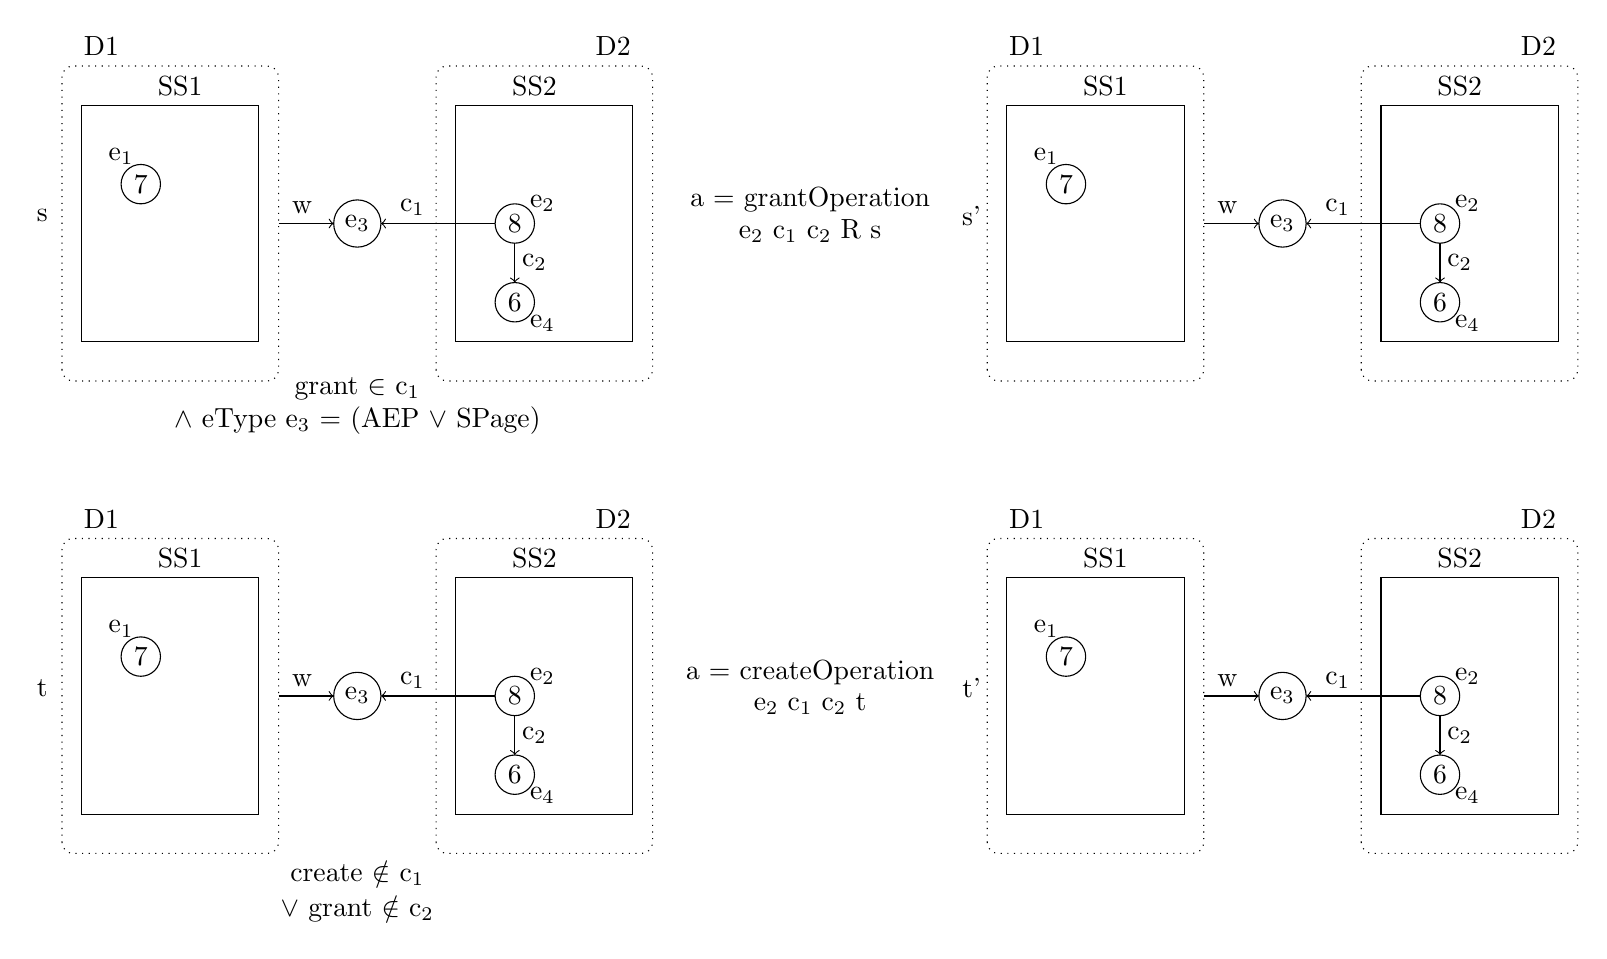
\begin{tikzpicture}
\node at (-0.25,1.6) {t};
\node at (1.5,3.25) {SS1};
\node at (0.5,3.75) {D1};
\node at (7,3.75) {D2};
\draw [black, dotted, rounded corners] (0,-0.5) rectangle (2.75,3.5);
\draw [black] (0.25,0) rectangle (2.5,3);
\draw [black, dotted, rounded corners] (4.75,-0.5) rectangle (7.5,3.5);
\draw [black] (5,0) rectangle (7.25,3);
\draw [black] (1,2) circle [radius=0.25] node {7};
\node at (0.75,2.35) {e$_1$};
\node at (6,3.25) {SS2};
\node at (6.1,1.75) {e$_2$};
\node at (6.1,0.23) {e$_4$};
\draw [black] (5.75,1.5) circle [radius=0.25] node {8};
\draw [black] (5.75,0.5) circle [radius=0.25] node {6};
\draw [black, ->] (5.75,1.25)--(5.75,0.75);
\node at (6,1){c$_2$};
\node at (3.75,-0.75) {create $\notin$ c$_1$};
\node at (3.75,-1.2) {$\vee$ grant $\notin$ c$_2$};
\node at (9.5,1.8) {a = createOperation};
\node at (9.5,1.4) { e$_2$ c$_1$ c$_2$ t};
\draw [black] (3.75,1.5) circle [radius=0.3] node {e$_3$};
\draw [->, black] (2.75,1.5) -- (3.45,1.5);
\draw [<-, black] (4.05,1.5) -- (5.5,1.5);
\node at (3.05,1.7) {w};
\node at (4.45,1.7) {c$_1$};

\node at (11.55,1.6) {t'};
\node at (12.25,3.75) {D1};
\node at (18.75,3.75) {D2};
\node at (13.25,3.25) {SS1};
\draw [black, dotted, rounded corners] (11.75,-0.5) rectangle (14.5,3.5);
\draw [black] (12,0) rectangle (14.25,3);
\draw [black, dotted, rounded corners] (16.5,-0.5) rectangle (19.25,3.5);
\draw [black] (16.75,0) rectangle (19,3);
\draw [black] (12.75,2) circle [radius=0.25] node {7};
\node at (12.5,2.35) {e$_1$};
\node at (17.75,3.25) {SS2};
\node at (17.85,1.75) {e$_2$};
\node at (17.85,0.23) {e$_4$};
\draw [black] (17.5,1.5) circle [radius=0.25] node {8};
\draw [black] (17.5,0.5) circle [radius=0.25] node {6};
\draw [->, black] (17.5,1.25)--(17.5,0.75);
\node at (17.75,1){c$_2$};
\draw [black] (15.5,1.5) circle [radius=0.3] node {e$_3$};
\draw [->, black] (14.5,1.5) -- (15.2,1.5);
\draw [<-, black] (15.8,1.5) -- (17.25,1.5);
\node at (14.8,1.7) {w};
\node at (16.2,1.7) {c$_1$};

\node at (-0.25,7.6) {s};
\node at (1.5,9.25) {SS1};
\node at (0.5,9.75) {D1};
\node at (7,9.75) {D2};
\draw [black, dotted, rounded corners] (0,5.5) rectangle (2.75,9.5);
\draw [black] (0.25,6) rectangle (2.5,9);
\draw [black, dotted, rounded corners] (4.75,5.5) rectangle (7.5,9.5);
\draw [black] (5,6) rectangle (7.25,9);
\draw [black] (1,8) circle [radius=0.25] node {7};
\node at (0.75,8.35) {e$_1$};
\node at (6,9.25) {SS2};
\node at (6.1,7.75) {e$_2$};
\node at (6.1,6.23) {e$_4$};
\draw [black] (5.75,7.5) circle [radius=0.25] node {8};
\draw [black] (5.75,6.5) circle [radius=0.25] node {6};
\draw [black, ->] (5.75,7.25)--(5.75,6.75);
\node at (6,7){c$_2$};
\node at (3.75,5.4) {grant $\in$ c$_1$};
\node at (3.75,5) {$\wedge$ eType e$_3$ = (AEP $\vee$ SPage)};
\node at (9.5,7.8) {a = grantOperation}; 
\node at (9.5,7.4) {e$_2$ c$_1$ c$_2$ R s};
\draw [black] (3.75,7.5) circle [radius=0.3] node {e$_3$};
\draw [->, black] (2.75,7.5) -- (3.45,7.5);
\draw [<-, black] (4.05,7.5) -- (5.5,7.5);
\node at (3.05,7.7) {w};
\node at (4.45,7.7) {c$_1$};

\node at (11.55,7.6) {s'};
\node at (12.25,9.75) {D1};
\node at (18.75,9.75) {D2};
\node at (13.25,9.25) {SS1};
\draw [black, dotted, rounded corners] (11.75,5.5) rectangle (14.5,9.5);
\draw [black] (12,6) rectangle (14.25,9);
\draw [black, dotted, rounded corners] (16.5,5.5) rectangle (19.25,9.5);
\draw [black] (16.75,6) rectangle (19,9);
\draw [black] (12.75,8) circle [radius=0.25] node {7};
\node at (12.5,8.35) {e$_1$};
\node at (17.75,9.25) {SS2};
\node at (17.85,7.75) {e$_2$};
\node at (17.85,6.23) {e$_4$};
\draw [black] (17.5,7.5) circle [radius=0.25] node {8};
\draw [black] (17.5,6.5) circle [radius=0.25] node {6};
\draw [->, black] (17.5,7.25)--(17.5,6.75);
\node at (17.75,7){c$_2$};
\draw [black] (15.5,7.5) circle [radius=0.3] node {e$_3$};
\draw [->, black] (14.5,7.5) -- (15.2,7.5);
\draw [<-, black] (15.8,7.5) -- (17.25,7.5);
\node at (14.8,7.7) {w};
\node at (16.2,7.7) {c$_1$};
\end{tikzpicture}
\end{document}
